\chapter{Алгоритм на изогениях}
\label{ch:isogenies}

В этой главе будет рассмотрен принцип работы алгоритма SIDH (Supersingular Isogeny Diffie-Hellman).

\section{Изогении как математическая структура}

\subsection{Эллиптические кривые}

Изогении основаны на эллиптических кривых.

Нам понадобится сложение точек на эллиптических кривых (пример на Рисунке \ref{fig:elliptic_curve}) и определение порядка точки: $\deg P = n$, если $[n]P = \mathcal{O}$, где $[n]P$ -- сложение $P$ с самим собой $n$ раз, $\mathcal{O}$ -- нейтральный элемент .

\begin{figure}[ht]
	\centering
	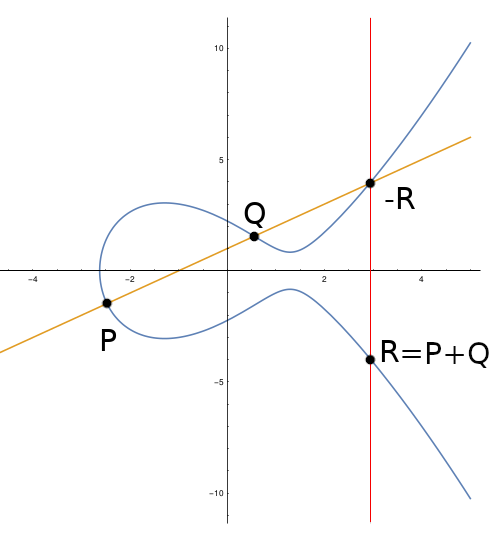
\includegraphics[width=0.5\textwidth]{elliptic_curve}
	\caption{Пример эллиптической кривой}
	\label{fig:elliptic_curve}
\end{figure}

Пусть дана $P \in E$, а точка $S$ вычисляется как $S = [n] P \in E$. 
Классическая задача (используемая в EdDSA) -- дискретный логарифм на эллиптических кривых, ставится так: найти $n$ такое, что $S = [n] P$.

Эта задача сложная для классических компьютеров, но не для квантовых.

\subsection{Изоморфизмы и $j$-инварианты}

С этого момента будем работать в поле $\mathds{F}_{q^2}.$

Для эллиптической кривой $E_a$ можно ввести понятие $j$-инварианта -- специальное число, описывающее данную кривую. Например, для кривой $E_a: y^2 = x^3 + ax^2 + x$ $j$-инвариант задается как $j(E_a) = \frac{256(a^3-3)^3}{a^2-4}$.

Кривые $E$ и $E'$ называются изоморфными ($E \cong E'$), если у них одинаковые $j$-инварианты. Между любыми изоморфными кривыми существует линейное преобразование $\psi$, переводящее одну кривую в другую. Соответственно, существует и обратное ему $\psi^{-1}$:

\begin{equation*}
	\begin{aligned}
		& \psi      &: E \rightarrow E', \qquad & (x, y) \rightarrow (\alpha x + \beta, \gamma y), \\
		& \psi^{-1} &: E' \rightarrow E, \qquad & (x, y) \rightarrow (\alpha' x + \beta', \gamma' y).
	\end{aligned}
\end{equation*}

Заметим, что у них отсутствуют особые точки, то есть $\ker \psi = \{ \mathcal{O}_E \}$, $\ker \psi = \{ \mathcal{O}_E' \}$, где $\mathcal{O}$ -- нейтральный элемент группы.

\subsection{Изогении}

В случае, когда $j$-инварианты не равны, мы можем строить нелинейные отображения. Для некоторых пар $E$, $E'$ у отображений появляются нули в знаменателе. У этих отображений $\ker \varphi$ нетривиален. Тогда $E$ и $E'$ называются изогенными друг другу, а отображение $\varphi$ называется изогенией.

Для любого конечного подмножества $G$ точек на $E$ существует единственная изогения $\varphi$, для которой $\ker \varphi = G$. Формулы Велу (Vélu's formulas) по $G$ вычисляют $\varphi$ и $E'$ \cite{velu_elliptic}.

Композиция изогений сохраняет групповые свойства:
\begin{equation*}
	\varphi(P + Q) = \varphi(P) + \varphi(Q).
\end{equation*}
Размер ядра $\varphi$ будем называть его степенью: $\deg \varphi = \# (\ker \varphi)$. Для композиции изогений существует свойство:
\begin{equation*}
	\deg (\varphi_1 \circ \varphi_2) = \deg(\varphi_1) \cdot \deg(\varphi_2).
\end{equation*}

Таким образом, мы можем строить изогении очень высокого порядка как цепочку композиций изогений малого порядка.

\subsection{Упрощаем начальные условия}

1) Для всех изогений, полученных по формулам Велу выполняется свойство:
\begin{equation*}
	(x, y) \rightarrow (f(x),\; cyf'(x)), \quad c = \text{const}.
\end{equation*}
Поэтому мы можем опускать $y$ в дальнейших выкладках.

2) Для алгоритма требуются изогении порядков $n = 2$ и $n = 3$.

\section{Операции агентов}

Операции агентов достаточно сложны и требуют выкладок в области теории групп. Общая идея заключается в разложении изогении высокого порядка на многократную композицию изогений малых порядков \cite{isogenies}.

\section{Граф $j$-инвариантов}

Для любого простого числа $p$ в поле $\mathds{F}_{p^2}$ существует около $p/12$ особых эллиптических кривых (с точностью до гомоморфизма), которые позволяют ввести на них группу относительно умножения. Каждой из них соответствуют значение $j$-инварианта. На Рисунке \ref{fig:isogenies} приведен пример для $p = 431$ \cite{isogenies}.

\begin{figure}[ht]
	\centering
	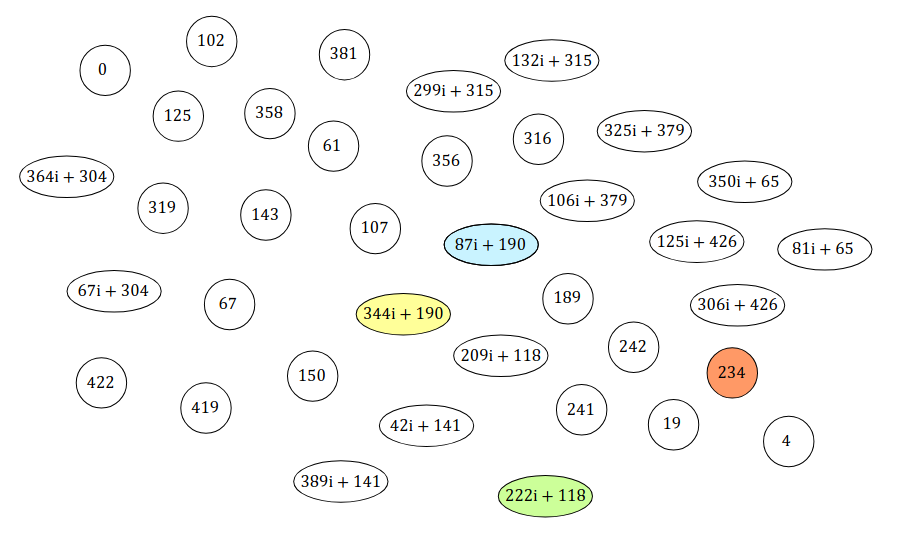
\includegraphics[width=0.7\textwidth]{isogenies}
	\caption{Пример графа для $p=431$}
	\label{fig:isogenies}
\end{figure}

Операции каждого из агентов создают различный набор дуг, которые соединяют узлы графа $j$-инвариантов. Они изображены на Рисунках \ref{fig:isogenies_a} и \ref{fig:isogenies_b}.

\begin{figure}[ht]
	\centering
	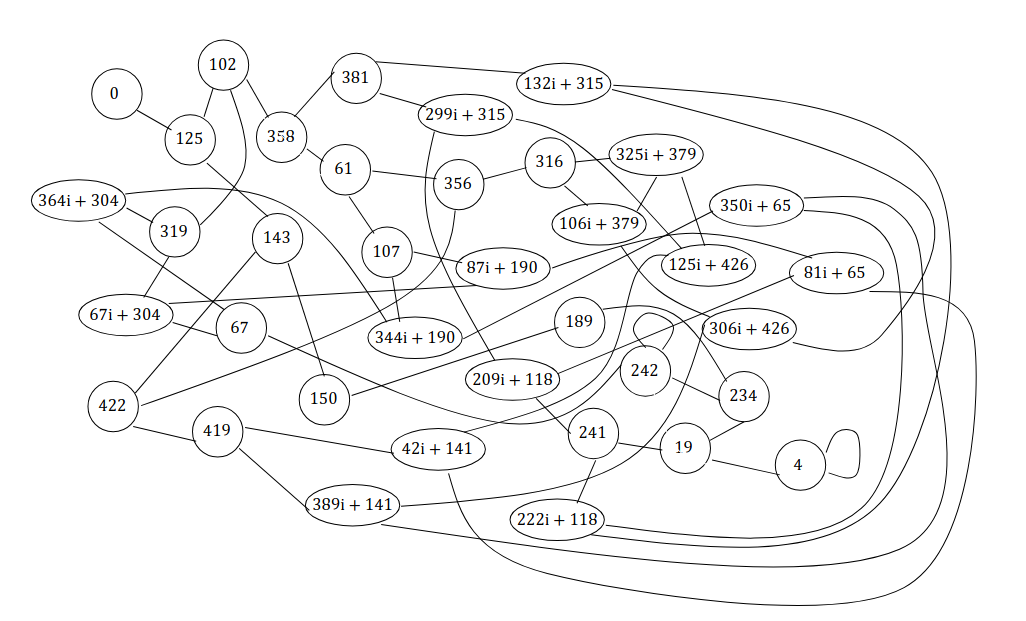
\includegraphics[width=0.7\textwidth]{isogenies_a}
	\caption{Граф агента А, связанный изогениями второго порядка (по три ребра из каждой вершины)}
	\label{fig:isogenies_a}
\end{figure}

\begin{figure}[ht]
	\centering
	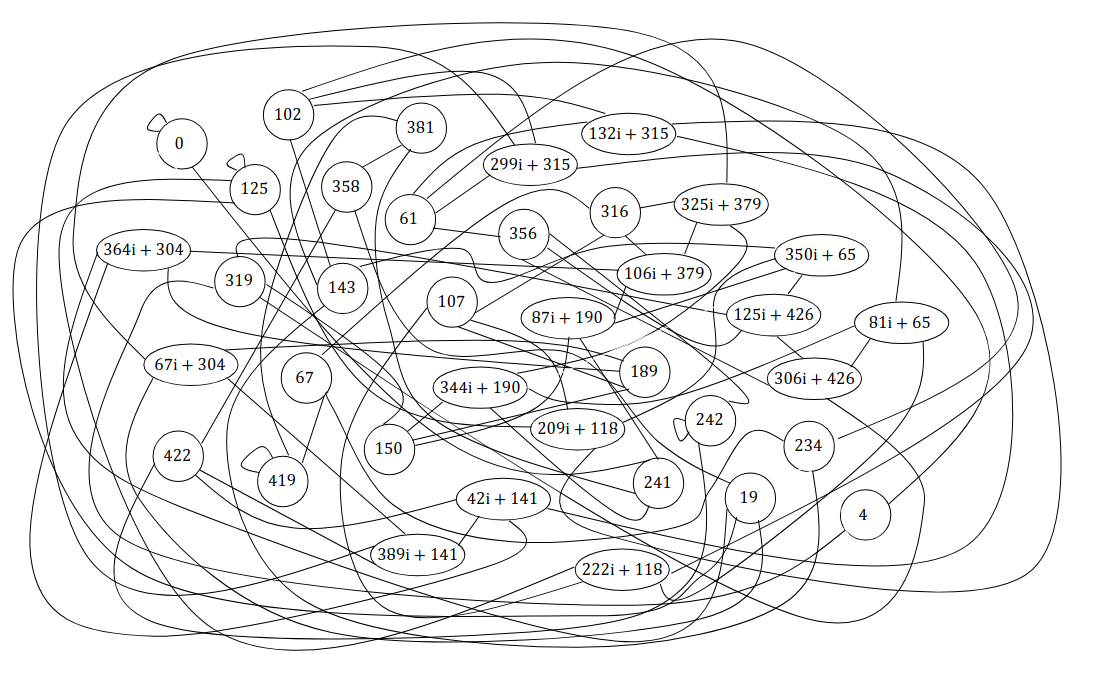
\includegraphics[width=0.7\textwidth]{isogenies_b}
	\caption{Граф агента Б, связанный изогениями третьего порядка (по четыре ребра из каждой вершины)}
	\label{fig:isogenies_b}
\end{figure}

Важно отметить, что для любого $p$ как бы мы не переставляли узлы, схема связей останется сложной. Это свойство отображает возможность добраться от одного узла до другого за малое число шагов.

Еще одним важным свойством является независимость полученных графов двух агентов.

Простое число $p$ выбирается особым образом:
\begin{equation*}
	p = 2^k 3^m - 1.
\end{equation*}
При этом числа $k$ и $m$ задают количество изогений (шагов в графе), которые совершат агенты А и Б, соответственно.

\section{Движение до открытого ключа}

В качестве начальных условий выступает $E_a$ -- некоторая эллиптическая кривая, задающая начальный $j$-инвариант.

Рассмотрим движение агента А по графу. Он выбирает точку $S$ порядка $\deg S = 2^4 = 16$.

На первом шаге он выполняет следующую последовательность операций:
\begin{equation*}
	S \rightarrow [2]S \rightarrow [4]S \rightarrow [8]S
\end{equation*}
\begin{equation*}
	\varphi_0: \ker \varphi_0 = \{ \mathcal{O}, [8]S \}.
\end{equation*}
Так он получает изогению $\varphi_0$ для перехода в другой узел.

Второй шаг:
\begin{equation*}
	S \rightarrow \varphi_0(S) \rightarrow [2] \varphi_0(S) \rightarrow [4] \varphi_0(S)
\end{equation*}
\begin{equation*}
	\varphi_0: \ker \varphi_1 = \{ \mathcal{O}, [4]\varphi_0(S) \}.
\end{equation*}
Так он получает следующую изогению $\varphi_1$ для перехода.

\begin{figure}[ht]
	\centering
	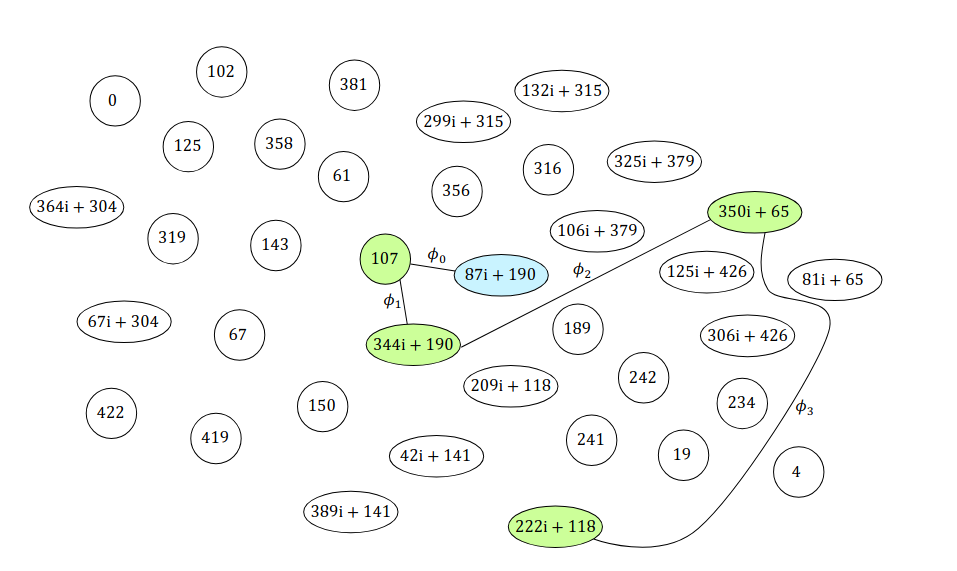
\includegraphics[width=0.7\textwidth]{steps_a}
	\caption{Шаги агента А}
	\label{fig:steps_a}
\end{figure}

Третий шаг:
\begin{equation*}
	S \rightarrow \varphi_0(S) \rightarrow \varphi_1(\varphi_0(S)) \rightarrow [2] \varphi_1(\varphi_0(S))
\end{equation*}
\begin{equation*}
	\varphi_2: \ker \varphi_2 = \{ \mathcal{O}, [2]\varphi_1(\varphi_0(S)) \}.
\end{equation*}

Четвертый шаг:
\begin{equation*}
	S \rightarrow \varphi_0(S) \rightarrow \varphi_1(\varphi_0(S)) \rightarrow \varphi_2(\varphi_1(\varphi_0(S)))
\end{equation*}
\begin{equation*}
	\varphi_3: \ker \varphi_3 = \{ \mathcal{O}, \varphi_2(\varphi_1(\varphi_0(S))) \}.
\end{equation*}

Агент Б проводит аналогично 3 шага с $\deg S = 27$, $[3]$ и $deg \varphi_i = 3$.

\begin{figure}[ht]
	\centering
	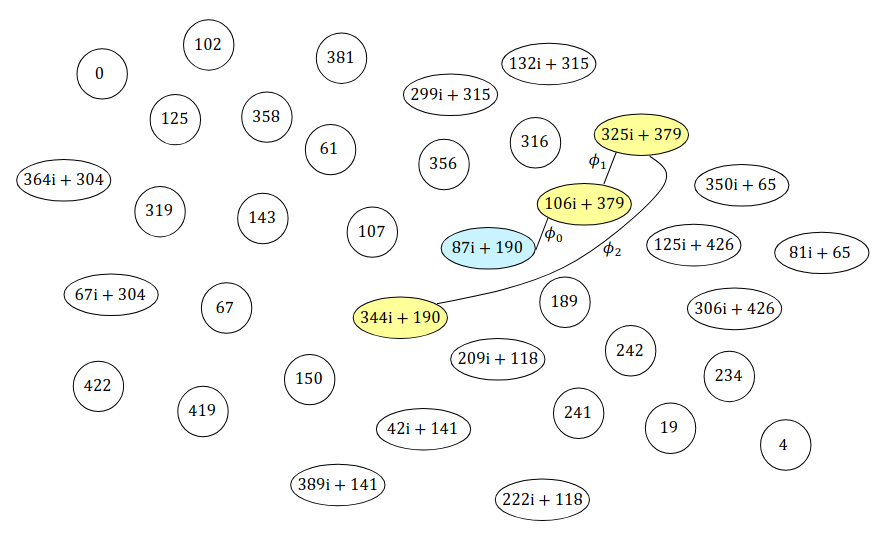
\includegraphics[width=0.7\textwidth]{steps_b}
	\caption{Шаги агента Б}
	\label{fig:steps_b}
\end{figure}

По итогу каждый из агентов получает $\{ S, \varphi_0, ... \varphi_m \}$ -- закрытый ключ, а также итоговый узел $E_n$ -- открытый ключ.

\section{Движение до общего секретного ключа}

Агенты А и Б передают друг другу их открытые ключи -- новые начальные узлы в графе. Они проводят точно такое же движение по графу, но уже с новых узлов.

\begin{figure}[ht]
	\centering
	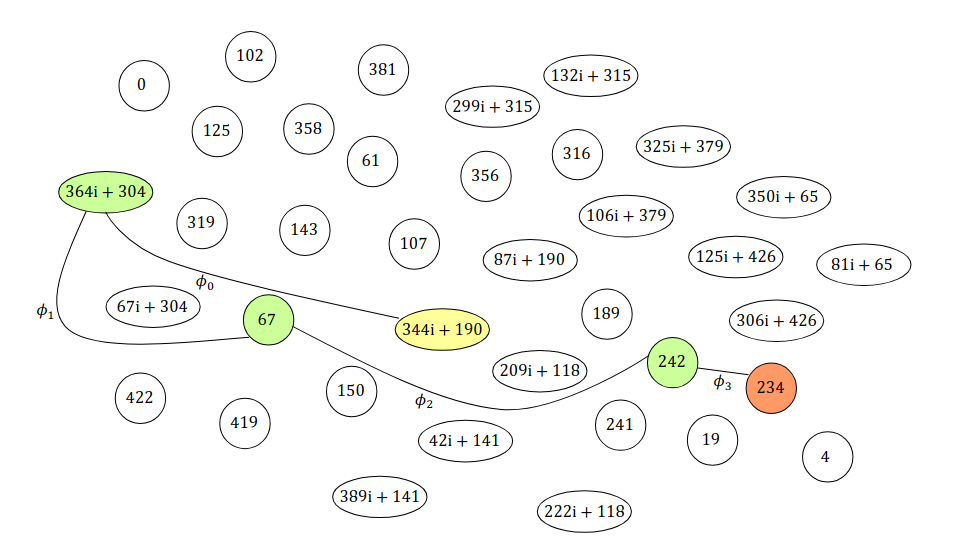
\includegraphics[width=0.7\textwidth]{secret_a}
	\caption{Шаги агента А}
	\label{fig:secret_a}
\end{figure}

\begin{figure}[ht]
	\centering
	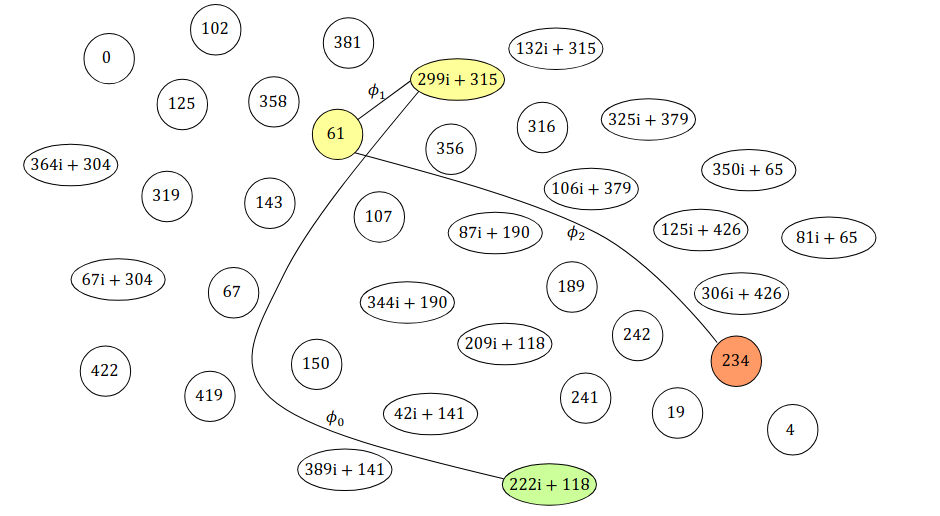
\includegraphics[width=0.7\textwidth]{secret_b}
	\caption{Шаги агента Б}
	\label{fig:secret_b}
\end{figure}

Все эти построения приводят А и Б к общему узлу. При этом злоумышленник имеет лишь начальный узел и два открытых ключа. Изогении, приводящие к этому ключу, получены как композиция большого количества изогений малого порядка. Они имеют очень высокую степень, а сложность поиска обратного пути экспоненциально растет с порядком изогении \cite{isogenies}.

\endinput
